% !TeX spellcheck = russian-aot-ieyo
% Зачем: Определяет класс документа (То, как будет выглядеть документ)
% Примечание: параметр draft помечает строки, вышедшие за границы страницы, прямоугольником, в фильной версии его нужно удалить.
\documentclass[a4paper,14pt,russian,oneside,final]{article}

% Зачем: Настройка Times New Roman.

% Рекомендовано для Linux (нужен scalable-cyrfonts-tex, подробности см. в fonts_linux.tex)
% раскомментировать, чтобы использовать:
% Зачем: Выбор внутренней TeX кодировки.
\usepackage[T2A]{fontenc}

% Зачем: Предоставляет свободный Times New Roman.
% Шрифт идёт вместе с пакетом scalable-cyrfonts-tex в Ubuntu/Debian

% пакет scalable-cyrfonts-tex может конфликтовать с texlive-fonts-extra в Ubuntu
% решение: Для себя я решил эту проблему так: пересобрал пакет scalable-cyrfonts-tex, изменив его имя. Решение топорное, но работает. Желающие могут скачать мой пакет здесь:
% https://yadi.sk/d/GW2PhDgEcJH7m
% Установка:
% dpkg -i scalable-cyrfonts-tex-shurph_4.16_all.deb

\usefont{T2A}{ftm}{m}{sl}

% Зачем: Установка кодировки исходных файлов.
\usepackage[utf8]{inputenc}

% Зачем: Делает результирующий PDF "searchable and copyable".
\usepackage{cmap}

% Зачем: Чтобы можно было использовать русские буквы в формулах, но в случае использования предупреждать об этом.
\usepackage[warn]{mathtext}

% Зачем: Учет особенностей различных языков.
\usepackage[russian]{babel}

% Зачем: Добавляет поддержу дополнительных размеров текста 8pt, 9pt, 10pt, 11pt, 12pt, 14pt, 17pt, and 20pt.
% Почему: Пункт 2.1.1 Требований по оформлению пояснительной записки.
\usepackage{extsizes}


% Зачем: Длинна, пимерно соответвующая 5 символам
% Почему: Требования содержат странное требование про отсупы в 5 символов (для немоноширинного шрифта :| )
\newlength{\fivecharsapprox}
\setlength{\fivecharsapprox}{6ex}


% Зачем: Добавляет отступы для абзацев.
% Почему: Пункт 2.1.3 Требований по оформлению пояснительной записки.
\usepackage{indentfirst}
\setlength{\parindent}{\fivecharsapprox} % Примерно соответсвует 5 символам.


% Зачем: Настраивает отступы от границ страницы.
% Почему: Пункт 2.1.2 Требований по оформлению пояснительной записки.
\usepackage[left=3cm,top=2.0cm,right=1.5cm,bottom=2.7cm]{geometry}


% Зачем: Настраивает межстрочный интервал, для размещения 40 +/- 3 строки текста на странице.
% Почему: Пункт 2.1.1 Требований по оформлению пояснительной записки.
\usepackage[nodisplayskipstretch]{setspace} 
\setstretch{1.5}
%\onehalfspacing

% Зачем: Выбор шрифта по-умолчанию. 
% Почему: Пункт 2.1.1 Требований по оформлению пояснительной записки.
% Примечание: В требованиях не указан, какой именно шрифт использовать. По традиции используем TNR.
\renewcommand{\rmdefault}{ftm} % Times New Roman


% Зачем: Отключает использование изменяемых межсловных пробелов.
% Почему: Так не принято делать в текстах на русском языке.
\frenchspacing


% Зачем: Добавляет скобку 1) к номеру сноски
% Почему: Пункты 2.9.2 и 2.9.1 Требований по оформлению пояснительной записки.
\makeatletter 
\def\@makefnmark{\hbox{\@textsuperscript{\normalfont\@thefnmark)}}}
\makeatother


% Зачем: Расположение сносок внизу страницы
% Почему: Пункт 2.9.2 Требований по оформлению пояснительной записки.
\usepackage[bottom]{footmisc}

% Зачем: Переопределяем стандартную нумерацию, т.к. в отчете будут только section и т.д. в терминологии TeX
\makeatletter
\renewcommand{\thesection}{\arabic{section}}
\makeatother


% Зачем: Пункты (в терминологии требований) в терминологии TeX subsubsection должны нумероваться
% Почему: Пункт 2.2.3 Требований по оформлению пояснительной записки.
\setcounter{secnumdepth}{3}


% Зачем: Настраивает отступ между таблицей с содержанимем и словом СОДЕРЖАНИЕ
% Почему: Пункт 2.2.7 Требований по оформлению пояснительной записки.
\usepackage{tocloft}
\setlength{\cftbeforetoctitleskip}{-1em}
\setlength{\cftaftertoctitleskip}{1em}


% Зачем: Определяет отступы слева для записей в таблице содержания.
% Почему: Пункт 2.2.7 Требований по оформлению пояснительной записки.
\makeatletter
\renewcommand{\l@section}{\@dottedtocline{1}{0.5em}{1.2em}}
\renewcommand{\l@subsection}{\@dottedtocline{2}{1.7em}{2.0em}}
\makeatother


% Запрещаем перенос слов
\hyphenpenalty=10000
\tolerance=400
\emergencystretch=3em


% Зачем: Задает стиль заголовков раздела жирным шрифтом, прописными буквами, без точки в конце
% Почему: Пункты 2.1.1, 2.2.5, 2.2.6 и ПРИЛОЖЕНИЕ Л Требований по оформлению пояснительной записки.
\makeatletter
\renewcommand\section{%
  \clearpage\@startsection {section}{1}%
    {\fivecharsapprox}%
    {-1em \@plus -1ex \@minus -.2ex}%
    {1em \@plus .2ex}%
    {\centering\hyphenpenalty=10000\normalfont\large\bfseries}}
\makeatother


% Зачем: Задает стиль заголовков подразделов
% Почему: Пункты 2.1.1, 2.2.5 и ПРИЛОЖЕНИЕ Л Требований по оформлению пояснительной записки.
\makeatletter
\renewcommand\subsection{%
  \@startsection{subsection}{2}%
    {\fivecharsapprox}%
    {-1em \@plus -1ex \@minus -.2ex}%
    {1em \@plus .2ex}%
    {\centering\hyphenpenalty=10000\normalfont\normalsize\bfseries}}
\makeatother


% Зачем: Задает стиль заголовков пунктов
% Почему: Пункты 2.1.1, 2.2.5 и ПРИЛОЖЕНИЕ Л Требований по оформлению пояснительной записки.
\makeatletter
\renewcommand\subsubsection{
  \@startsection{subsubsection}{3}%
    {\fivecharsapprox}%
    {-1em \@plus -1ex \@minus -.2ex}%
    {0em}%
    {\raggedright\hyphenpenalty=10000\normalfont\normalsize\bfseries}}
\makeatother

% Зачем: для оформления введения и заключения, они должны быть выровнены по центру.
% Почему: Пункты 1.1.15 и 1.1.11 Требований по оформлению пояснительной записки.
\makeatletter
\newcommand\sectioncentered{%
  \clearpage\@startsection {section}{1}%
    {\z@}%
    {-1em \@plus -1ex \@minus -.2ex}%
    {1em \@plus .2ex}%
    {\centering\hyphenpenalty=10000\normalfont\large\bfseries\MakeUppercase}%
    }
\makeatother



% Зачем: Задает стиль библиографии
\bibliographystyle{ugost2003}

\makeatletter
\renewcommand\@biblabel[1]{#1.}
\makeatother


% Зачем: Пакет для вставки картинок
% Примечание: Объяснение, зачем final - http://tex.stackexchange.com/questions/11004/why-does-the-image-not-appear
\usepackage[final]{graphicx}
\DeclareGraphicsExtensions{.pdf,.png,.jpg,.eps}


% Зачем: Директория в которой будет происходить поиск картинок
\graphicspath{{pictures/}}


% Зачем: Добавление подписей к рисункам
\usepackage[nooneline]{caption}
\usepackage{subcaption}

% Зачем: чтобы работала \No в новых латехах
\DeclareRobustCommand{\No}{\ifmmode{\nfss@text{\textnumero}}\else\textnumero\fi}

% Зачем: поворот ячеек таблиц на 90 градусов
\usepackage{rotating}
\DeclareRobustCommand{\povernut}[1]{\begin{sideways}{#1}\end{sideways}}


% Зачем: когда в формулах много кириллических символов команда \text{} занимает много места
\DeclareRobustCommand{\x}[1]{\text{#1}}


% Зачем: Задание подписей, разделителя и нумерации частей рисунков
% Почему: Пункт 2.5.5 Требований по оформлению пояснительной записки.
\DeclareCaptionLabelFormat{stbfigure}{Рис. #2}
\DeclareCaptionLabelFormat{stbtable}{Таблица #2}
\DeclareCaptionLabelSeparator{stb}{~--~}
\captionsetup{labelsep=stb}
\captionsetup[figure]{labelformat=stbfigure,figurewithin=none,justification=centering}
\captionsetup[table]{labelformat=stbtable,justification=centering}
\renewcommand{\thesubfigure}{\asbuk{subfigure}}


% Зачем: Окружения для оформления формул
% Почему: Пункт 2.4.7 требований по оформлению пояснительной записки и специфические требования различных кафедр
% Пример использования смотри в course_content.tex, строка 5
\usepackage{calc}
\newlength{\lengthWordWhere}
\settowidth{\lengthWordWhere}{где}
\newenvironment{explanationx}
    {%
    %%% Следующие строки определяют специфические требования разных редакций стандартов. Раскоменнтируйте нужную строку
    %% стандартный абзац, СТП-01 2010
    %\begin{itemize}[leftmargin=0cm, itemindent=\parindent + \lengthWordWhere + \labelsep, labelsep=\labelsep]
    %% без отступа, СТП-01 2013
    \begin{itemize}[leftmargin=0cm, itemindent=\lengthWordWhere + \labelsep , labelsep=\labelsep]%
    \renewcommand\labelitemi{}%
    }
    {%
    %\\[\parsep]
    \end{itemize}
    }

% Старое окружение для "где". Сохранено для совместимости
\usepackage{tabularx}

\newenvironment{explanation}
    {
    %%% Следующие строки определяют специфические требования разных редакций стандартов. Раскоменнтируйте нужные 2 строки
    %% стандартный абзац, СТП-01 2010
    %\par 
    %\tabularx{\textwidth-\fivecharsapprox}{@{}ll@{ --- } X }
    %% без отступа, СТП-01 2013
    \noindent 
    \tabularx{\textwidth}{@{}ll@{ --- } X }
    }
    { 
    \\[\parsep]
    \endtabularx
    }


% Зачем: Удобная вёрстка многострочных формул, масштабирующийся текст в формулах, формулы в рамках и др
\usepackage{amsmath}


% Зачем: Поддержка ажурного и готического шрифтов 
\usepackage{amsfonts}


% Зачем: amsfonts + несколько сотен дополнительных математических символов
\usepackage{amssymb}


% Зачем: Окружения «теорема», «лемма»
\usepackage{amsthm}


% Зачем: Производить арифметические операции во время компиляции TeX файла
\usepackage{calc}

% Зачем: Производить арифметические операции во время компиляции TeX файла
\usepackage{fp}

% Зачем: Пакет для работы с перечислениями
\usepackage{enumitem}
\makeatletter
 \AddEnumerateCounter{\asbuk}{\@asbuk}{щ)}
\makeatother


% Зачем: Устанавливает символ начала простого перечисления
% Почему: Пункт 2.3.5 Требований по оформлению пояснительной записки.
\setlist{nolistsep}


% Зачем: Устанавливает символ начала именованного перечисления
% Почему: Пункт 2.3.8 Требований по оформлению пояснительной записки.
\renewcommand{\labelenumi}{\asbuk{enumi})}
\renewcommand{\labelenumii}{\arabic{enumii})}

% Зачем: Устанавливает отступ от границы документа до символа списка, чтобы этот отступ равнялся отступу параграфа
% Почему: Пункт 2.3.5 Требований по оформлению пояснительной записки.

\setlist[itemize]{leftmargin=0ex}
\setlist[itemize,0]{itemindent=\parindent + 2.2ex,leftmargin=0ex,label=--}
\setlist[enumerate,1]{itemindent=\parindent + 2.7ex,leftmargin=0ex}
\setlist[enumerate,2]{itemindent=\parindent + \parindent - 2.7ex}

% Зачем: Включение номера раздела в номер формулы. Нумерация формул внутри раздела.
%\AtBeginDocument{\numberwithin{equation}{section}}

% Зачем: Включение номера раздела в номер таблицы. Нумерация таблиц внутри раздела.
%\AtBeginDocument{\numberwithin{table}{section}}

% Зачем: Включение номера раздела в номер рисунка. Нумерация рисунков внутри раздела.
%\AtBeginDocument{\numberwithin{figure}{section}}


% Зачем: Дополнительные возможности в форматировании таблиц
\usepackage{makecell}
\usepackage{multirow}
\usepackage{array}


% Зачем: "Умная" запятая в математических формулах. В дробных числах не добавляет пробел
% Почему: В требованиях не нашел, но в русском языке для дробных чисел используется {,} а не {.}
\usepackage{icomma}

% Зачем: макрос для печати римских чисел
\makeatletter
\newcommand{\rmnum}[1]{\romannumeral #1}
\newcommand{\Rmnum}[1]{\expandafter\@slowromancap\romannumeral #1@}
\makeatother


% Зачем: Управление выводом чисел.
\usepackage{sistyle}
\SIdecimalsign{,}

% Зачем: inline-коментирование содержимого.
\newcommand{\ignore}[2]{\hspace{0in}#2}


% Зачем: Возможность коментировать большие участки документа
\usepackage{verbatim}


\usepackage[dvipsnames]{xcolor}


% Зачем: Оформление листингов кода
% Примечание: final нужен для переопределения режима draft, в котором листинги не выводятся в документ.
\usepackage[final]{listingsutf8}


% Зачем: настройка оформления листинга для языка F#
\definecolor{bluekeywords}{rgb}{0.13,0.13,1}
\definecolor{greencomments}{rgb}{0,0.5,0}
\definecolor{turqusnumbers}{rgb}{0.17,0.57,0.69}
\definecolor{redstrings}{rgb}{0.5,0,0}

\renewcommand{\lstlistingname}{Листинг}

\lstdefinelanguage{Kotlin}{
  keywords={package, as, typealias, this, super, val, var, fun, for, null, true, false, is, in, throw, return, break, continue, object, if, try, else, while, do, when, yield, typeof, yield, typeof, class, interface, enum, object, override, public, private, get, set, import, abstract, },
  keywordstyle=\color{NavyBlue}\bfseries,
  ndkeywords={@Deprecated, Iterable, Int, Integer, Float, Double, String, Runnable, dynamic},
  ndkeywordstyle=\color{BurntOrange}\bfseries,
  emph={println, return@, forEach,},
  emphstyle={\color{OrangeRed}},
  identifierstyle=\color{black},
  sensitive=true,
  commentstyle=\color{green}\ttfamily,
  comment=[l]{//},
  morecomment=[s]{/*}{*/},
  stringstyle=\color{ForestGreen}\ttfamily,
  morestring=[b]",
  morestring=[s]{"""*}{*"""},
  extendedchars=false
}

\lstdefinelanguage{Go} {
  % Keywords as defined in the language grammar
  morekeywords=[1]{%
    break,default,func,interface,select,case,defer,go,map,%
    struct,chan,else,goto,package,switch,const,fallthrough,%
    if,range,type, continue,for,import,return,var},
  % Built-in functions
  morekeywords=[2]{%
    append,cap,close,complex,copy,delete,imag,%
    len,make,new,panic,print,println,real,recover},
  % Pre-declared types
  morekeywords=[3]{%
    bool,byte,complex64,complex128,error,float32,float64,%
    int,int8,int16,int32,int64,rune,string,%
    uint,uint8,uint16,uint32,uint64,uintptr},
  % Constants and zero value
  morekeywords=[4]{true,false,iota,nil},
  keywordstyle=\color{NavyBlue}\bfseries,
  % Strings : "foo", 'bar', `baz`
  morestring=[b]{"},
  morestring=[b]{'},
  morestring=[b]{`},
  % Comments : /* comment */ and // comment
  comment=[l]{//},
  morecomment=[s]{/*}{*/},
  % Options
  sensitive=true,
  extendedchars=false
}

\lstdefinestyle{kotlinstyle}{
   xleftmargin=0ex,
   language=Kotlin,
   basicstyle=\footnotesize\ttfamily,
   breaklines=true,
   columns=fullflexible, keepspaces
}

\lstdefinestyle{gostyle}{
   xleftmargin=0ex,
   language=Go,
   basicstyle=\footnotesize\ttfamily,
   breaklines=true,
   columns=fullflexible, keepspaces
}

\lstdefinestyle{jstyle}{
   xleftmargin=0ex,
   basicstyle=\footnotesize\ttfamily,
   breaklines=true,
   columns=fullflexible, keepspaces
   extendedchars=false
}

% Зачем: Нумерация листингов в пределах секции
%\AtBeginDocument{\numberwithin{lstlisting}{section}}

\usepackage[normalem]{ulem}

\usepackage[final,hidelinks]{hyperref}
% Моноширинный шрифт выглядит визуально больше, чем пропорциональный шрифт, если их размеры одинаковы. Искусственно уменьшаем размер ссылок.
\renewcommand{\UrlFont}{\small\rmfamily\tt}

\usepackage[square,numbers,sort&compress]{natbib}
\setlength{\bibsep}{0em}

% Магия для подсчета разнообразных объектов в документе
\usepackage{lastpage}
\usepackage{totcount}
\regtotcounter{section}

\usepackage{etoolbox}


% Для оформления таблиц не влязящих на 1 страницу
\usepackage{longtable}

% Для включения pdf документов в результирующий файл
\usepackage{pdfpages}

% Для использования знака градуса и других знаков
% http://ctan.org/pkg/gensymb
\usepackage{gensymb}

% Зачем: преобразовывать текст в верхний регистр командой MakeTextUppercase
\usepackage{textcase}

% Зачем: Переносы в словах с тире.
% Тире в словае заменяем на \hyph: аппаратно\hyphпрограммный.
% https://stackoverflow.com/questions/2193307/how-to-get-latex-to-hyphenate-a-word-that-contains-a-dash#
\def\hyph{-\penalty0\hskip0pt\relax}

% Добавляем абзацный отступ для библиографии
% https://github.com/mstyura/bsuir-diploma-latex/issues/19
\setlength\bibindent{-1.0900cm}

\makeatletter
\renewcommand\NAT@bibsetnum[1]{\settowidth\labelwidth{\@biblabel{#1}}%
   \setlength{\leftmargin}{\bibindent}\addtolength{\leftmargin}{\dimexpr\labelwidth+\labelsep\relax}%
   \setlength{\itemindent}{-\bibindent+\fivecharsapprox-0.240cm}%
   \setlength{\listparindent}{\itemindent}
\setlength{\itemsep}{\bibsep}\setlength{\parsep}{\z@}%
   \ifNAT@openbib
     \addtolength{\leftmargin}{\bibindent}%
     \setlength{\itemindent}{-\bibindent}%
     \setlength{\listparindent}{\itemindent}%
     \setlength{\parsep}{10pt}%
   \fi
}



\newcommand{\csharp}{C\#}
\newcommand{\fsharp}{F\#}
\newcommand{\vbnet}{Visual Basic~.NET}
\newcommand{\cpp}{C\texttt{\hspace{-0.3ex}+\hspace{-0.25ex}+}}
\newcommand{\cppcli}{Visual \cpp{}/CLI}
\newcommand{\dotnet}{Microsoft .NET}
\newcommand{\netfx}{.NET Framework}
\newcommand{\java}{Java}

\begin{document}

%\begin{titlepage}
  \begin{center}
    Министерство образования Республики Беларусь\\[1em]
    Учреждение образования\\
    БЕЛОРУССКИЙ ГОСУДАРСТВЕННЫЙ УНИВЕРСИТЕТ \\
    ИНФОРМАТИКИ И РАДИОЭЛЕКТРОНИКИ\\[1em]

    \begin{minipage}{\textwidth}
      \begin{flushleft}
        \begin{tabular}{ l l }
          Факультет & Компьютерных систем и сетей\\
          Кафедра   & Информатики
        \end{tabular}
      \end{flushleft}
    \end{minipage}\\[1em]

    \begin{flushright}
      \begin{minipage}{0.4\textwidth}
        \textit{К защите допустить:}\\[0.8em]
        Заведующий кафедрой ПИКС\\[0.45em]
        \underline{\hspace*{2.8cm}} И.\,Н.~Цырельчук
      \end{minipage}\\[2.2em]
    \end{flushright}

    %%
    %% ВНИМАНИЕ: на некторых факультетах (ФКП) и кафедрах (ПИКС) слова "ПОЯСНИТЕЛЬНАЯ ЗАПИСКА" предлагается (требуется) оформлять полужирным начертанием. Раскомментируйте нужную для вас строку:
    %%
    %\textbf{ПОЯСНИТЕЛЬНАЯ ЗАПИСКА}\\
    {ПОЯСНИТЕЛЬНАЯ ЗАПИСКА}\\
    {к дипломному проекту}\\
    {на тему:}\\[1em]
    \textbf{\large АЛГОРИТМЫ ПОСТРОЕНИЯ ВЕРОЯТНОСТНЫХ СЕТЕЙ}\\[1em]


    {БГУИР ДП 1-31 03 04 07 093 ПЗ}\\[2em]
    
    \begin{tabular}{ p{0.65\textwidth}p{0.25\textwidth} }
      Студент & Ю.\,А.~Ярошевич \\
      Руководитель & А.\,А.~Волосевич \\
      Консультанты: &\\
      \hspace*{3ex}\emph{от кафедры информатики} & А.\,А.~Волосевич \\
      \hspace*{3ex}\emph{по экономической части} & А.\,В.~Рябов \\
      %%
      %% ВНИМАНИЕ: в зависимости от выбранной темы, у вас консультант может быть как по охране труда, так и по:
        % экологической безопасности
        % ресурсосбережению
        % энергосбережению
      %%
      %% Впишите правильную формулировку по необходимости
      \hspace*{3ex}\emph{по охране труда} & Е.\,А.~Колосова \\
      Нормоконтролёр & С.\,И.~Сиротко\\
      & \\
      Рецензент &
    \end{tabular}
    
    \vfill
    {\normalsize Минск 2013}
  \end{center}
\end{titlepage}
 % page 1


%\setcounter{page}{5}

% Зачем: Содержание пишется полужирным шрифтом, по центру всеми заглавными буквами
% Почему: Пункт 2.2.7 Требований по оформлению пояснительной записки.
\renewcommand \contentsname {\centerline{\bfseries\large{\MakeUppercase{содержание}}}}

% Зачем: Не захламлять основной файл
% Примечание: \small\selectfont злостный хак, чтобы уменьшить размер шрифта в ToC 
{
\normalsize\selectfont
\tableofcontents
\newpage
}

\sectioncentered*{Введение}
\addcontentsline{toc}{section}{ВВЕДЕНИЕ}

В настоящее время все более актуальной становится задача защиты информационных ресурсов компьютерных сетей от атак со стороны внутренних или внешних нарушителей. Это связано прежде всего со стремительным развитием информационных технологий, охватывающих многие сферы жизни общества и государства в целом. В повседневной жизни Интернет используется не только для сбора информации, но и для работы с централизованными базами данных, для работы с клиентами, для объединения филиалов и удаленных подразделений в единую сеть, и так далее. Поэтому в настоящее время остро стоят вопросы  эффективной и гибкой защиты ресурсов корпоративной сети организации при ее подключении к глобальной сети от внешних нарушителей и локальной сети при угрозе от внутренних нарушителей \citep{emelyanova_fralenko}.

Злоумышленник всегда первым выбирает цель и методы осуществления атаки, а система защиты не имеет информации о его выборе до тех пор, пока не будет зарегистрировано вторжение. Для решения данной проблемы необходимо не только предупреждать, блокировать, обнаруживать и реагировать на действия нарушителей, но и отвлекать их от основных целей, заманивая на ложные информационные объекты, производить сбор информации о приемах, тактике и мотивации злоумышленников, осуществлять их идентификацию и разоблачение. Именно поэтому все более актуальной задачей становится внедрение обманных систем в защищаемую сеть. Другими словами, такие ложные информационные системы или по-другому — обманные системы («ловушки») создаются для привлечения злоумышленников и удерживают их внимание на «приманке». А пока злоумышленник будет атаковать приманку вместо того, чтобы атаковать реальную сеть, установленные на ней средства слежения и регистрации должны будут зафиксировать все подробности этого процесса:  выявить атаки, направить их по ложному следу, ограничить их распространение, идентифицировать нарушителей, исследовать их действия и определить намерения.

Цель данной работы — разработать систему автоматизации процесса создания инфраструктуры обманной системы в корпоративной сети.

Для достижения данной цели были поставлены следующие задачи: 

\begin{itemize}
	\item разработать архитектуру системы автоматического разворачивания ловушек;
	\item определить механизм взаимодействия между компонентами системы;
	\item разработать математическую модель сети с целью последующей выработки механизма определения количества ловушек в системе и их характеристик;
	\item разработать систему автоматического разворачивания ловушек.
\end{itemize}

\section{Особенности применения обманных систем для обнаружения вторжений}

Обманная система (ОбС) представляют собой комплекс программно-аппаратных средств обеспечения информационной безопасности, реализующая функции сокрытия защищаемых информационных ресурсов, а также дезинформации нарушителей. С помощью фиксации, сбора данных, и обмана нарушителей (на основе имитации ложных целей, уязвимых для нападения), а также других механизмов эти системы позволяют в реальном времени выявлять атаки, направлять их по ложному следу, ограничивать их распространение, идентифицировать нарушителей, исследовать их действия и определять намерения \citep{Kotenko2014}.

Обманная система состоит из элементов, называемых ловушками, приманками или honeypot. Ловушка — это ресурс, задача которого подвергнуться атаке или несанкционированному исследованию. Помимо ловушек, обманная система должна включать в себя системы сбора и хранения данных и системы управления. 

Обманные системы предназначены для реализации следующих основных целей:
\begin{itemize}
\item ограничение атак на целевые (критически важные) системы за счет отвлечения нарушителя и “принятия огня на себя” (следствием чего является снижение эффективности атак, в том числе замедление их реализации, или их полное блокирование; это может позволить вовремя среагировать на распространение вирусов, сетевых червей и т.п.);
\item скрытное обнаружение (отслеживание) и исследование (оперативный анализ) атак и не авторизованной активности (издержки сокращаются за счет снижения числа ложных срабатываний, так как любой трафик, направленный на обманную систему вероятнее всего содержит действия нарушителя); 
\item мониторинг случаев несанкционированного доступа к системе и ее использования не по назначению;
\item реагирование на действия нарушителя с целью введения его в заблуждение \citep{Kotenko2014} \citep{Hernacki2004}.
\end{itemize}

Обманная система не должна участвовать в повседневной работе корпоративной сети, к ней не должно происходить каких-либо обращений от других узлов, за исключением подключений с целью администрирования. По данной причине обманная система имеет низкую вероятность ложных срабатываний, так как любое обращение будет расцениваться как неправомерное.

Обманная система не предпринимает активных действий по привлечению злоумышленника. Реагирование на действия нарушителя происходит только после его непосредственной атаки.

Одной из главных особенностей применения обманных систем является сложность выбора конфигурации \citep{rajan}. Настройка ОбС является нетривиальной задачей. Количество, расположение и конфигурацию ловушек необходимо выбирать так, чтобы их применение было максимально эффективным.

\subsection{Особенности реализации сетей приманок}

Под фактической реализацией сетей приманок понимается выбор технологий управления ложными целями в составе обособленного сегмента сети, а также конкретные алгоритмы функционирования всех подсистем ОбС.  Независимо от используемых при реализации ловушек технологий, обманная система в обязательном порядке должна содержать определенные  компоненты для полноценной работы.

\subsubsection{Система сбора и хранения данных}\hspace*{\fill}

Обманная система должна содержать систему сбора и хранения данных о деятельности злоумышленника в системе, в том числе о командах, инициированных им. Нарушители могут использовать шифрование, чтобы скрыть свои действия. Например, как только нарушитель проник на хост обманной системы, он может осуществлять удаленное администрирование системы с помощью \textit{SSH}.

Для решения этой проблемы можно использовать специальные модули ядра операционной системы, устанавливаемые на хостах, которые могут стать объектами атак. Эти модули накапливают информацию обо всей деятельности нарушителей. Информацию, которую собирают модули ядра, нельзя сохранять локально на хосте, поскольку возникает угроза обнаружения, удаления или модификации этой информации. 

Возникает необходимость удаленно собирать на защищенной системе, причем так, чтобы нарушитель об этом не знал. От компонентов обманной системы требуется передавать собранную информацию в сеть. Однако злоумышленник может проанализировать трафик и обнаружить, что в пересылаемых пакетах содержатся сведения о его собственной деятельности. Чтобы воспрепятствовать этому, компонент должен маскировать пакеты, например, под трафик \textit{NetBIOS}, передаваемый из других систем. Причем \textit{IP} и \textit{MAC} адреса отправителей и получателей могут маскироваться под адреса локального сервера \textit{Windows}, а данные, содержащиеся в пакетах, — шифроваться. В этом случае даже если нарушитель осуществляет перехват и анализ пакетов, то для него они будут выглядеть как обычный трафик.

\subsubsection{Система восстановления и создания резервных копий}\hspace*{\fill}

Обманная система, как и любая другая структура в сфере информационных технологий, постоянно изменяется с течением времени. Добавления новых компонентов, изменения конфигурации существующих, поломки в результате критических ситуаций обязательно присутствуют в ее жизненном цикле.

Обнаружение новых уязвимостей в компонентах корпоративной сети также оставляет свой след и на элементах обманной системы. Данные моменты влекут за собой необходимость включения системы восстановления и создания резервных копий. 

Наличие резервных копий позволяет восстановить состояние ловушки в исходное после повреждения в результате атаки, безопасно производить ее модификацию. Благодаря им появляется возможность быстрого переноса обманной системы или дублирования ее компонентов.

Наличие резервной копии ловушки, полученной после проведения атаки, существенно упрощает процесс анализа, позволяет определить инструментарий злоумышленника, выявить его намерения и детально изучить следы его деятельности. Таким образом данная система позволяет создать образ поврежденного элемента для последующего его анализа в лабораторных условиях.

\subsubsection{Система удаленного управления состояния ловушки}\hspace*{\fill}

Изменения рабочих процессов, расширение штата сотрудников, процедуры увеличения производительности системы и многое другое приводят к необходимости модифицирования компьютерной сети. Любое добавление, удаление или изменение узла или хранящейся на нем информации может повлиять на оптимальность текущей конфигурации обманной системы и требует изменения расположения ловушек. В условиях больших масштабов предприятия данные модификации происходят достаточно часто, поэтому в случае ручного режима работы с обманной системой возникает потребность в человеческих ресурсах, затраты по которым практически сравнимы с добавлением нового сетевого узла. Таким образом, система удаленного управления, позволяющая производить добавление новых или удаления старых ловушек очевидно не является необходимой, но строго рекомендуемой. Система автоматизации позволит минимизировать риск того, что необходимые изменения будут отложены по вине человеческого фактора, а также существенно упростит жизнь системному администратору и специалисту по безопасности.

\subsection{Существующие реализации обманных систем}

В настоящее время существует несколько реализаций обманных систем. Наиболее известными являются \citep{honeynet}:
\begin{itemize}
\item \textit{Capture-HPC}
\item \textit{Dionaea}
\item \textit{Dockpot}
\item \textit{Glastopf}
\item \textit{HIHAT}
\item \textit{HoneyC}
\item \textit{Honeyd}
\item \textit{Honeymole}
\item \textit{Honeystick}
\end{itemize}

Большинство перечисленных реализаций не получили своего распространения по причине достаточно сложного процесса настройки или большого количества требований к окружению. Остальные решения, не смотря на низкий порог вхождения, не предоставляют той гибкости, которая необходима для комфортной интеграции и использования. К примеру \textit{Honeyd} достаточно прост в конфигурации и не требователен к своему окружению, предоставляет дистрибутивы как для \textit{UNIX}, так и для \textit{Windows} систем, однако его концепция изначально являлась весьма сомнительной: \textit{Honeyd} позволяет эмулировать компьютерную сеть из нескольких ловушек, однако эмуляция производиться на одном хосте и нет возможности построения распределенной обманной системы.

Также ни один инструмент не предоставляет функционала подбора конфигурации обманной системы. Все реализации представляют собой конечный вариант ловушки, задача настройки которой остается на стороне пользователя.

Важным фактом является то, что ни одна из перечисленных систем не имеет поддержки со стороны разработчиков на данный момент, что сразу уменьшает степень доверия к инструментам со стороны потенциальных клиентов.

Компании, специализирующиеся на разработке систем защиты от киберугроз и анализе уязвимостей, также используют обманные системы в своей работе. К примеру "Лаборатория Касперского" оценивает степень ориентированности атак на устройства из систем \textit{IoT} при помощи установленных в глобальной сети Интернет ловушек, эмулирующих работу умных часов, \textit{smart TV}, роутеров, камер и других элементов Интернета Вещей \citep{kaspersky}. Однако данные разработки являются закрытыми коммерческими проектами и не представлены огласке.

Таким образом можно сделать вывод, что подходящего инструмента, позволяющего развернуть распределенную обманную систему в корпоративную сеть с малыми ручными затратами, и распространяющегося открытым либо коммерческим способом на данный момент не существует.

\section{Архитектура системы автоматического разворачивания ОбС}

Прежде чем выделять компоненты системы и рассматривать варианты их взаимодействия необходимо перечислить основные требования, возлагаемые на разрабатываемую систему:
\begin{itemize}
\item ловушки должны будут функционировать на реальных хостах сети с целью исключения аппаратных затрат;
\item при изменениях топологии защищаемой сети необходимо без больших затрат по времени и ресурсам изменять количество и расположение ловушек. Следует учесть, что под топологией подразумевается не только логическая топология сети, но и особенности расположения в ней таких важных функциональных элементов, как: почтовые сервера, сервера баз данных и приложений, сервера печати и т.д.;
\item необходим процесс создания и восстановления резервных копий ловушек;
\item необходим мониторинг активности запущенных ловушек и удаленный съем информации в случае возникновения на них активности.
\end{itemize}

Из перечисленных требований следует факт необходимости централизованного управления и распределенного функционирования разрабатываемой системы. Таким образом, разрабатываемая система будет в обязательном порядке содержать два компонента:
\begin{itemize}
	\item компонент централизованного управления, далее называемый <<центральный узел>>;
	\item компонент для обслуживания ловушки на конечном хосте, выполняющий операции изменения ее состояния по команде от первого компонента. Далее данный компонент будет называться <<агент>>.
\end{itemize}


\subsection{Выбор технологии для создания и разворачивания ловушек}

С учетом требования на запуск ловушек на реальных хостах сети, удобнее всего применять технологии виртуализации, которые позволяют использовать ресурсы одного физического сервера для создания нескольких виртуальных хостов.

В условиях большого количества ловушек актуальной является задача уменьшения потребления вычислительных ресурсов виртуальной машиной, поэтому целесообразно рассматривать технологии контейнерной виртуализации \citep{Joy2015}. При данной технологии ядро операционной системы поддерживает несколько изолированных экземпляров пространства пользователя, вместо одного. Эти экземпляры с точки зрения пользователя полностью идентичны реальному серверу. Для систем на базе \textit{UNIX}, эта технология может рассматриваться как улучшенная реализация механизма \textit{chroot}. Наиболее популярной системой контейнерной виртуализации является \textit{LXC} \citep{lxc_doc}, однако использование ее в чистом виде несет за собой массу неудобств, поэтому следует рассматривать инструменты, позволяющие упростить работу с \textit{LXC} контейнерами.

С недавнего времени технологии контейнерной виртуализации стали неотъемлемым инструментом в процессе разработки и поставки программного обеспечения, так как позволяют существенно упростить создание необходимого окружения для выполнения поставляемого приложения. Тот факт, что среда, в которой приложение разрабатывается, будет соответствовать среде эксплуатации вдохновило \textit{IT} индустрию на создание вспомогательных инструментов для автоматизации работы с виртуализацией на уровне операционной системы.

Несомненным фаворитом среди контейнерных систем является \textit{Docker}.

\textit{Docker} является программным обеспечением для автоматизации процессов разворачивания и управления приложением в среде виртуализации на уровне операционной системы, позволяет упаковывать приложение со всем необходимым окружением в контейнер и предоставляет программный интерфейс для его управления. Данное ПО прекрасно подходит на роль инструмента для создания ловушек, так как является активно поддерживаемым и предоставляет большое количество готовых контейнеров посредством облачной системы \textit{Docker Hub}.

Перечислим особенности данного программного обеспечения, которые покрывают некоторые требования к разрабатываемой системе \citep{Boettiger2015}:

\begin{itemize}
\item  \textit{docker} контейнер может быть перезапущен без сохранения своего состояния. Благодаря данному факту отпадает необходимость в восстановлении и создании резервных копий, так как сам по себе \textit{docker} образ является резервной копией, а восстановление осуществляется  операцией пересоздания контейнера из образа;
\item  простой механизм задания конфигурации для \textit{docker} образа. Детали окружения запускаемых в контейнере приложений, а также непосредственно множество приложений с параметрами их запуска описываются в одном конфигурационном файле. Параметры сети и объемы выделяемых под контейнер ресурсов указываются в команде запуска контейнера;
\item  программный интерфейс \textit{Docker} предоставляет команды для отслеживания и съема изменений в системе контейнера.
\end{itemize}

С учетом перечисленных особенностей можно сделать вывод о том, что \textit{Docker} является подходящим инструментом для разрабатываемой системы.

Для каждой ловушки необходимо сформировать соответствующий docker образ, который будет содержать в себе все необходимые для ее работы компоненты. В задачи системы автоматизации разворачивания будет входить назначение соответствующего образа на заданный хост в компьютерной сети и последующий запуск контейнера.

\subsection{Агенты}

В компьютерной сети могут находиться узлы, которые не обладают достаточными ресурсными возможностями для запуска на ней контейнера с ловушкой. Факт обладания такими возможностями не может быть обнаружен автоматически и задача выделения хостов является задачей системного администратора.

На доступных к разворачиванию контейнеров хостах системному администратору необходимо будет установить агента, в обязанности которого будут входить:

\begin{itemize}
\item копирование необходимого \textit{docker} образа с указанного ресурса;
\item изменение состояния \textit{docker} контейнера по команде от некоторого центрального узла;
\item мониторинг активности в запущенном контейнере и информирование центрального узла в случае ее возникновения;
\item передача информации о состоянии контейнера центральному узлу при получении соответствующих запросов.
\end{itemize}

Наличие агента на хосте не говорит о наличии на нем ловушки. Агент выступает посредником между центральным узлом и приманкой, сам по себе потребляет минимальное количество ресурсов и, в случае отключенной ловушки, никаким образом не влияет на производительность.

Совокупность всех агентов в сети определяет подмножество узлов, на которых обманная система может производить необходимые операции. В случае изменения назначения узлов достаточно удаления агента из системы автоматизации и с обслуживаемого хоста.

Единственным требованием выдвигаемым к хосту является наличие на нем установленного дистрибутива \textit{Docker}, необходимого для функционирования ловушки.

Таким образом алгоритм внедрения системы автоматического разворачивания состоит из следующих шагов:

\begin{itemize}
	\item системный администратор выделяет узлы компьютерной сети, ресурсные возможности которого позволяют запустить на них ловушки;
	\item выделяется хост под центральный узел;
	\item на каждый выделенный администратором узел устанавливаются агент и, по необходимости, \textit{Docker}, настраивается соединение с центральным узлом.
\end{itemize}


\subsection{Центральный узел}

В обязанности центрального узла системы, как управляющего агентами компонента, будут входить следующие пункты:

\begin{enumerate}
	\item регистрирование добавленных агентов в системе;
	\item мониторинг активности агента, в который входят следующие проверки:
		\begin{enumerate}
			\item проверка доступности агента;
			\item проверка работоспособности хоста в случае отсутствия связи с установленным на нем агентом. Случай, в котором с агентом отсутствует соединение, но соответствующий хост является доступным, считается критичным;
			\item получение состояния контейнера на агенте. Возможны три варианта состояния: отключен, включен и активность отсутствует, включен и активность присутствует.	
		\end{enumerate}
	\item управление состоянием контейнера на агенте. Предусматривается следующий набор команд:
		\begin{enumerate}
			\item задание другого \textit{docker} образа на агента;
			\item запуск назначенного контейнера с указанными параметрами;
			\item отключение запущенного контейнера;
		\end{enumerate}
	\item прием от агента и последующее сохранение информации об активности в контейнере.
\end{enumerate}

Помимо перечисленного, центральный узел должен на основании топологии компьютерной сети и расположения доступных агентов предоставлять пользователю потенциально наиболее оптимальное расположение и конфигурации ловушек.

\section{Коммуникация между элементами системы автоматического разворачивания ОбС}

Одной из основных проблем функционирования распределенной обманной системы с множеством ловушек является задача скрытой коммуникации между элементами обманной системы \citep{Peskova2014}. Информацию, собранную о деятельности злоумышленника внутри ловушки-контейнера, нецелесообразно хранить как в самом контейнере, так и на хосте, поддерживающем его функционирование. Возникает угроза компрометации: злоумышленник может обнаружить, удалить и модифицировать данную информацию. Исходя из сказанного следует факт необходимости удаленного сбора. 

Внедрение удаленного сбора информации влечет за собой требования к должной защите данной коммуникации от перехвата. Злоумышленник может проанализировать трафик и обнаружить, что в пересылаемых пакетах содержатся сведения о его собственной деятельности. Можно выделить два способа решения описанной проблемы:
\begin{enumerate}
	\item исключить возможность перехвата пересылаемых данных;
	\item исключить возможность получения информации из пакетов, в случае их перехвата.
\end{enumerate}

Первый способ решения имеет большое количество проблем в реализации. Следует учитывать, что, потенциально, объем передаваемой информации будет достаточно велик. Злоумышленник может производить большое количество действий в контейнере, которые будут порождать массовые изменения в его файловой системе. Все произведенные действия и их результаты необходимо будет передавать на центральный узел. Существующие на данный момент способы скрытой передачи имеют слабую пропускную способность, поскольку базируются либо на стеганографических методах, либо используют встраивание в существующие протоколы (ICMP, IGMP, NetBIOS и т.д.) и не гарантируют полной защиты от перехвата.

Таким образом остается вариант предупреждения возможности получения информации из перехваченных пакетов путем шифрования.

\subsection{Выбор протокола коммуникации}

Учитывая особенности коммуникации между агентом и центральным узлом, наиболее подходящим способом ее реализации является создание своего протокола прикладного уровня, удовлетворяющего специфическим требованиям. Однако реализация своего протокола несет за собой высокую долю вероятности содержания ошибок, поэтому более целесообразным  решением является выбор подходящего протокола прикладного уровня среди существующих.

Требования к соединению между агентом и центральным узлом:
\begin{enumerate}
\item поддержка шифрования;
\item высокая пропускная способность;
\item выбранный протокол взаимодействия должен иметь активную поддержку со стороны команды разработки.
\end{enumerate}

Высокая пропускная способность обусловлена необходимостью к передаче данных малых и средних объемов. Вероятность того, что злоумышленник будет загружать или модифицировать файлы значительного размера крайне мала. В случае, если произойдет изменение файла большого объема, достаточно будет отключить автоматическую отправку с целью исключения затраты ресурсов на передачу и предоставления возможности для отправки других файлов.

Требование к активной поддержке объясняется своевременным реагированием высококвалифицированных специалистов на выявление в протоколе различного рода уязвимостей. Если используемый протокол будет актуален, сравнительно молод и широко распространен, то ему будет уделяться большое количество внимания со стороны информационного сообщества.

Перечисленным требованиям удовлетворяет протокол WebSocket. Перечислим преимущества использования данного протокола \citep{Fedorenkov2015WebSocket}:
\begin{itemize}
\item поддерживает криптографические протоколы SSL/TLS;
\item позволяет организовать полнодуплексную модель связи;
\item имеет низкие требование к сетевым ресурсам и высокую производительность передачи данных. Служебная информация составляет 2 байта на одно сообщение. По результатам сравнения\citep{Fedorenkov2015WebSocket} производительности передачи 1000, 10000 и 100000 пустых сообщений в секунду при помощи протоколов \textit{http} и \textit{WebSocket}, график которого представлен на рис. \ref{fig:websocket_http_compare}, можно сделать вывод, что в сравнении с протоколом \textit{http} протокол \textit{WebSocket} практически в 1000 раз меньше нагружает сеть;
\item протокол является широко используемым. Первая версия протокола вышла в 2008 году, доработан в 2010 и получил распространение в 2011 году. Данный пункт удовлетворяет третьему требованию.
\end{itemize}

\begin{figure}[ht]
\centering
	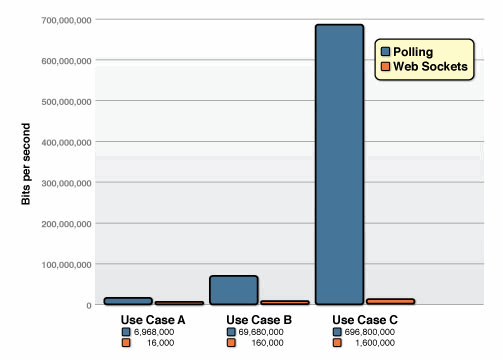
\includegraphics[scale=0.8]{websocket.png}  
	\caption{ Сравнение необходимой пропускной способности сети при передачи пустого сообщения при
помощи обычного \textit{http} соединения и при помощи вебсокетов}
	\label{fig:websocket_http_compare}
\end{figure}

\subsection{Защита коммуникации}

Выбранный протокол коммуникации поддерживает SSL шифрование. В системе будут использоваться два сертификата:
\begin{enumerate}
\item самоподписанный сертификат, закрытый ключ которого будет храниться вне корпоративной сети мероприятия с целью исключения возможности его фальсификации;
\item сертификат центрального узла, который будет использоваться при передаче информации между агентом и центральным узлом. Данный сертификат будет подписан первым сертификатом.
\end{enumerate}

Первый сертификат будет добавлен в агентов в качестве корневого доверенного сертификата.

С целью аутентификации подключаемого к центральному узлу агента   в момент его подключения в начале соединения будет передаваться некоторый секрет. Также данная мера позволяет отслеживать попытки анализа центрального узла со стороны злоумышленника.

Рассмотрим возможные направления развития ситуации:
\begin{itemize}
\item злоумышленник осуществил проникновение в корпоративную сеть и осуществляет перехват пакетов. Учитывая применение шифрования, он не сможет получить их содержимое, однако устанавливает факт необычной передачи данных. При попытке подключения к центральному узлу с целью выявления назначения сервиса и характера пересылаемых пакетов, злоумышленник не сможет пройти процедуру аутентификации, так как не знает необходимого секрета;
\item злоумышленник осуществил проникновение в корпоративную сеть и пытается осуществить MITM атаку с целью выявления секрета. Учитывая использование криптографического протокола SSL, который обеспечивает аутентификацию, проведение атаки MITM невозможно;
\item злоумышленник осуществил проникновение в корпоративную сеть и скомпрометировал хост, содержащий в себе агента, тем самым получив доступ к секрету и исполняемому файлу. Учитывая его информированность о структуре обманной системы ему нецелесообразно выдавать себя за один из ее элементов.
\end{itemize}

Исходя из рассмотренных ситуаций можно сделать вывод о том, что выбранный способ защиты является достаточным в рамках разрабатываемой системы.

\section{Автоматизация определения конфигурации обманной системы}

Одной из главных особенностей применения обманных систем является сложность выбора конфигурации \citep{rajan}. Количество, расположение и конфигурацию ловушек необходимо выбирать так, чтобы их применение было максимально эффективным. Для автоматизации данного процесса необходимо свести топологическую и функциональную модели защищаемой сети к некоторой математической модели. Она позволит применять существующие методы для решения поставленной задачи.

\subsection{Математическая модель защищаемой сети}

Предлагается исходить из следующих основных предположений:
\begin{itemize}
	\item для защищаемой сети актуальны атаки направленного типа;
	\item в сети выделяются две особые группы узлов: узлы, обрабатывающие критическую информацию, и узлы, непосредственно доступные для воздействия потенциального нарушителя;
	\item сеть обладает связностью, то есть из любой ее точки можно передать данные в любую другую точку за конечное число шагов;
	\item направленная атака представляет собой последовательность промежуточных (частных) атак, первая из которых имеет своей целью один из доступных нарушителю до начала атаки узлов, а последняя – один из узлов, работающих с критической информацией;
	\item система защиты информации не имеет достоверных сведений о начале направленной атаки, динамике ее развития, точном списке целей злоумышленника;
	\item нарушитель в начале направленной атаки не имеет достоверных сведений о структуре сети, однако может полностью или частично восстанавливать ее в ходе своих действий.
\end{itemize}

Система защиты должна быть спроектирована таким образом, чтобы вероятность контакта нарушителя с элементами обманной системы была максимально возможной.

Пусть $V$ — множество всех сетевых узлов, включающее как реальные, так и ложные цели. В соответствии с принятыми предположениями целью злоумышленника в ходе реализации направленной атаки является получение доступа к данным, хранящимся на определенных сетевых узлах в критических областях сети $V_{cr} \subset V$. Должен учитываться тот факт, что не все узлы одинаково доступны злоумышленнику и что на разных этапах атаки он может атаковать различные подмножества. Пусть $V_{avail,i} \subset V, i \in [0, k]$ - множество узлов, доступных нарушителю для атаки на шаге с номером $i$. Множество $V_{avail,0}$ является множеством потенциальных точек входа злоумышленника в сеть.

Неоднородность сети, вследствие которой множества $V_{avail,0}, ... , V_{avail,k}$ вообще говоря не совпадают между собой, обусловлена принимаемыми в сети мерами разграничения доступа, которые могут быть реализованы, например, в виде правил межсетевого экрана. Обычно правила разграничения сетевого доступа задаются при помощи дискреционной модели. В этом случае каждому узлу сети $v \in V$ можно поставить в соответствие список доступа $A_v = \{ w \in V | w \sim v \}$, где запись $w \sim v$ означает возможность прямой передачи данных между узлами $v$ и $w$.
 
Рассмотрим бинарное отношение $T$, заданное на множестве узлов сети: $T: V \times V \rightarrow \{0, 1\}$ по следующему правилу:
\begin{equation}
\label{eq:bin_network}
T(v_1, v_2) = 
	\begin{cases} 
		1,  & A_{v_1} = A_{v_2} \\
		0,  & A_{v_1} \neq A_{v_2} 
	\end{cases}
\end{equation}

Очевидно, отношение (\ref{eq:bin_network}) является отношением эквивалентности на множестве сетевых узлов. Классы эквивалентности, порожденные им (\ref{eq:netw_split}), обладают следующими свойствами: 

\begin{itemize}
	\item все узлы, входящие в один и тот же класс, одинаково доступны для атаки из всех точек сети;
	\item захват контроля над любым узлом в пределах одного класса дает возможность атаковать одни и те же цели;
	\item между любыми двумя узлами одного класса возможен прямой обмен данными.
\end{itemize}
\begin{equation}
\label{eq:netw_split}
V = V_1 \cup V_2 \cup ... \cup V_n
\end{equation}

На практике такие классы соответствуют областям сети с одинаковой политикой доступа. В случае использования межсетевого экрана в качестве средства разграничения доступа описанные выше классы эквивалентности принято называть зонами межсетевого экрана.

Поскольку направленная атака описывается последовательностью атакуемых узлов, ее можно однозначно задать с помощью последовательности $\sigma = V_{f_1}, V_{f_2}, ... , V_{f_k}$ зон, через которые нарушитель проходит в рамках атаки.

Взаимную доступность сетевых узлов, находящихся в разных зонах, удобно представлять в виде графа $G = (V, E)$, построенного по следующим правилам:

\begin{itemize}
	\item каждая вершина графа соответствует одной из зон межсетевого экрана;
	\item ребро графа проводится между двумя вершинами, если существует возможность прямой передачи данных между узлами в соответствующих зонах.
\end{itemize}

Обычно, если передача данных возможна в одном направлении, то она возможна и в обратном. Поэтому граф полагается ненаправленным.

Итак, поведение нарушителя в ходе направленной атаки может быть представлено в виде маршрута $\sigma$ в графе $G$. Этим маршрутом определяется порядок прохождения нарушителя через зоны межсетевого экрана. В каждой зоне межсетевого экрана, наряду с реальными, могут размещаться и ложные цели, входящие в состав обманной системы. Нарушитель не может с определенностью утверждать для каждого узла сети, является ли этот узел ложной целью или нет. Это приводит к тому, что при прохождении каждой из зон межсетевого экрана нарушитель может с некоторой вероятностью $P_{honey}$ совершить атаку на элемент ОбС.

Рассмотрим случай, когда все узлы одной зоны имеют одинаковую конфигурацию. Вероятность проведения атаки на элемент ОбС при прохождении зоны $V_{f_i}$ составляет $P_{honey} = l_i / s_i$, где $l_i, s_i$ - количество ложных целей и общее количество узлов в зоне $V_{f_i}$.

Рассмотрим некоторую направленную атаку, представимую в виде маршрута $\sigma = V_{f_1}, V_{f_2}, ... , V_{f_k}$. Вероятность того, что при прохождении некоторой зоны  контакт злоумышленника с ОбС будет отсутствовать составляет $ 1 - l_i / s_i$. Таким образом, вероятность того, что злоумышленник в результате проведения атаки  не попадет на элементы обманной системы составляет:
\begin{equation}
P_{victim} = \prod_{i=1}^k (1 - \frac{l_i}{s_i})
\end{equation}

Соответственно вероятность того, что злоумышленник в результате проведения атаки осуществит контакт с элементом обманной системы составляет:
\begin{equation}
\label{eq:p_honey}
P_{honey} = 1 - \prod_{i=1}^k (1 - \frac{l_i}{s_i})
\end{equation}

Каждый элемент произведения (\ref{eq:p_honey}) представляет собой вероятность контакта нарушителя и ОбС на одном из шагов направленной атаки. Заменим неориентированный граф $G$ на взвешенный ориентированный, проведя дуги в обоих направлениях между всеми инцидентными вершинами исходного графа . Каждой дуге, входящей в вершину $v$, соответствующей некоторой зоне $V_{f_i}$, поставим в соответствие число $w = 1 - l_i / s_i$, равное вероятности прохождения нарушителем области сети  без его обнаружения.

В рамках заданной математической модели задача о нахождении количества, расположения и конфигурации ловушек сводится к нахождению такого распределения элементов обманной сети по вершинам графа $G$, при котором максимизируется минимально возможная вероятность контакта злоумышленника с элементами обманной системы при проведении направленной атаки. Минимально возможная вероятность рассчитывается:
\begin{equation}
\label{eq:p_honey_min}
P_{honey, min} = \min_{\sigma \in S} P_{honey, \sigma} 
\end{equation}
где $S$ - множество всех возможных направленных атак на критические области $V_{cr}$.

Описанная модель работает в условиях, когда все узлы одной зоны имеют одинаковую конфигурацию. Данная модель расширяется до модели с поддержкой различных конфигураций следующим образом: каждую зону можно разбить на множества узлов с одинаковой конфигурацией
\begin{equation}
\label{eq:multi_conf}
V_{i} = V_i^{c_1} \cup V_i^{c_2} \cup ... \cup V_i^{c_m}, c_j \in C
\end{equation}
где $C$ - множество всех различных конфигураций в защищаемой сети.

Таким образом, всякой последовательности сетевых узлов можно поставить в соответствие последовательность множеств $V_i^{c_j}$. От графа $G$ можно перейти к графу $G'$, в котором вершинами являются множества узлов , при этом множество ребер преобразуется следующим образом:

\begin{itemize}
	\item в множестве $\{V_i^{c_{j_1}},..., V_i^{c_{j_k}}\}, V_i^{c_{j_l}} \neq \emptyset$, которое является разбиением типа (\ref{eq:multi_conf}) узла, соответствующему зоне $V_i$, присутствуют связи между каждой парой элементов;
	\item в случае наличия в графе $G$ ребра между узлами, соответствующими зонам $V_i$ и $V_j$, в графе $G'$ будут добавлены ребра для каждого множества из разбиений $V_i$ и $V_j$ типа (\ref{eq:multi_conf});
	\item веса ребер рассчитываются аналогично графу $G$.
\end{itemize}

Таким образом выработанная математическая модель защищаемой сети поддерживает возможность задания различных конфигураций.

\subsection{Решение оптимизационной задачи распределения ловушек}

Задача о нахождении количества, расположения и конфигурации ловушек свелась к оптимизационной задачи с целевой функцией задаваемой формулой (\ref{eq:p_honey_min}).

Существует большое количество способов решения оптимизационной задачи при помощи эвристических методов. В данной работе будет использоваться метод решения при помощи генетических алгоритмов.

Генетический алгоритм при помощи последовательных преобразований, схожих с процессами в модели биологической эволюции, над множеством промежуточных решений осуществляет поиск экстремумов заданной целевой функции. Для решения полученной оптимизационной задачи будет использоваться алгоритм \textit{NSGAII}. 

Данный алгоритм ориентирован на решение мультикритериальных задач, однако его концепция подходит и для решения однокритериальной задачи. \textit{NSGAII} при помощи специальных операторов селекции и дополнительного шага вытеснения доминирующих решений позволяет поддерживать равномерную с точки зрения целевой функции плотность популяции, обеспечивая таким образом более равномерную сходимость \citep{NSGA2002}.

Для применения выбранной реализации генетического алгоритма необходимо решить следующие подзадачи:
\begin{itemize}
	\item определить способ кодирования решения;
	\item сформировать целевую функцию и определить способ ее вычисления по заданному решению;
	\item выбрать операторы скрещивания и мутации.
\end{itemize}

\subsubsection{Кодирование решения}\hspace*{\fill}

По выработанной математической модели фактическое распределение элементов обманной системы определяется количеством ловушек присутствующих в каждой зоне $V_i, i=1..n$ из разбиения (\ref{eq:netw_split}). Таким образом распределению ловушек можно поставить в соответствие целочисленный вектор-хромосому (\ref{eq:solution}).
\begin{equation}
\label{eq:solution}
D = (h_1,h_2,...,h_n) 
\end{equation}
\begin{explanation}
где & $n$ & количество зон из разбиения (\ref{eq:netw_split});\\
	& $h_i$ & количество ловушек в зоне $V_i$.
\end{explanation}


\subsubsection{Целевая функция}\hspace*{\fill}

Полученная целевая функция (\ref{eq:p_honey_min}) определяет минимально возможную вероятность контакта злоумышленника с элементами обманной системы, однако в распределении ловушек присутствует еще такой важный фактор как количество задействованных агентов. Необходимо по возможности сокращать количество ловушек в системе для уменьшения потребления ресурсов с сохранением максимально возможного значения $P_{honey, min}$. Данный фактор можно выделить как отдельный критерий, однако технологии мультикритериальной оптимизации нацелены на получение множества компромиссных с точки зрения заданных критериев решений. В рассматриваемом случае ситуация обратная: в первую очередь необходимо максимизировать значение вероятности и только среди множества решений с максимально возможным значением вероятности выбирать решение с минимальным количеством задействованных ловушек. Для решения данной проблемы необходимо объединить оба критерия в одну скалярную функцию.

Значение (\ref{eq:p_honey_min}) лежит в диапазоне $[0, 1]$, при этом данную вероятность можно рассматривать с некоторой точностью до $k$ знаков после запятой. В рамках данной модели достаточно принять $k$ равное $5$, так как общее количество узлов $s_i$ в некоторой зоне $V_j$ на практике практически всегда меньше 10000, поэтому изменение в распределении ловушек  даже в случае столь крупных зон обязательно затронет более старшие знаки.

Таким образом целевая функция будет иметь вид (\ref{eq:fitness}).

\begin{equation}
\label{eq:fitness}
f(D) = (1 - \min_{\sigma \in S} P_{honey, \sigma}) + 10^{-5} \sum_{i=1}^n h_i
\end{equation}
\begin{explanation}
где & $D$ & распределение ловушек (\ref{eq:solution}); \\
	& $S$ & множество всех возможных направленных атак на критические области $V_{cr}$. \\
\end{explanation}

Значение $\min_{\sigma \in S} P_{honey, \sigma}$ было инвертировано в формуле целевой функции для упрощения расчета значения второго слагаемого.

Таким образом перед генетическим алгоритмом будет стоять задача по минимизации значения целевой функции $f(D)$.

Слагаемое с вероятностью рассчитывается при помощи алгоритмов поиска минимального маршрута на графах, в частности при помощи алгоритма Дейкстры.

\subsubsection{Выбор операторов генетического алгоритма}\hspace*{\fill}

Так как оператор селекции определен непосредственно в алгоритме \textit{NSGAII}, то необходимо задать операторы скрещивания и мутации.

Классические операторы скрещивания, производимые путем операции сечения хромосом и их последующей конкатенации, плохо применимы для данной оптимизационной задачи. На значение целевой функции влияет то подмножество элементов вектора решений, которое сформировывает наименее опасный для злоумышленника маршрут, и скрещивание путем склеивания некоторых подпоследовательностей из векторов родителей непосредственно влияют на него, в следствие чего на выходе получается некоторе случайное решение, непохожее на своих предков. Данный факт противоречит принципам оператора скрещивания, при применении которого получившееся решение должно забирать характерные признаки от своих родителей, но по возможности не совпадать ни с одним из них.


В качестве оператора скрещивания был выбран следующий вариант: для двух родителей $D_1 = (h_1^1, h_2^1, ..., h_n^1)$ и $D_2 = (h_1^2, h_2^2, ..., h_n^2)$ происходит поэлементное сравнение сравнение и соответствующее значение $h_i$ для генерируемого потомка $D_{1+2}$ рассчитывается следующим образом:
\begin{equation}
\label{eq:crossingover}
h_i(r) = max(0, \frac{h_i^1 + h_i^2}{2} + r * |h_i^1 - h_i^2|)
\end{equation}
где $r$ ---  некоторое случайное значение из диапазона $[-1,1]$.

Оператор (\ref{eq:crossingover}) характерен тем, что отличие элемента в векторе потомка тем меньше, чем более схожие распределения в рассматриваемых зонах у родителей, что обеспечивает более равномерную сходимость алгоритма.

В качестве оператора мутации использовался классический оператор, который случайным образом модифицирует некоторое случайное количество элементов вектора.

\begin{equation}
\label{eq:mutation}
h_i(r_1, r_2) =
\begin{cases}
	h_i & r_1 \geq 0.5 \\
	min(max(0, h_i + r_2), a_i) & r_1 < 0.5
\end{cases}
\end{equation}
\begin{explanation}
где & $r_1$ & некоторое случайное значение из диапазона $[0,1]$;\\
	& $r_2$ & некоторое случайное значение из диапазона $[-q,q]$;\\
	& $a_i$ & количество установленных агентов в зоне $V_i$.
\end{explanation}

Диапазон для $r_2$ регулирует интенсивность воздействия оператора мутации. Чем шире данный диапазон, тем больше результат оператора может отличаться от входного решения.

Значение диапазона было получено эмпирическим способом. Из формулы (\ref{eq:mutation}) следует, что рассматривать диапазоны, границы  которых превышают по модулю количество установленных агентов в зоне, не имеет смысла, поэтому перебор осуществлялся по $\{ [-q, q]\}_{q=1..k}$, где $k=\max_{i=1..n} a_i$.

Оценка эффективности работы алгоритма на конкретном наборе производится по моменту сходимости. За момент сходимости берется номер итерации алгоритма на котором было получено решение с минимальным значением целевой функции.

Оценка эффективности работы алгоритма с заданным значением $q$ производится путем получения минимального, максимального и среднего значений эффективности алгоритма на всем наборе тестовых конфигураций.

Эксперимент проводился по нескольким типам сети с различным количеством зон. Для каждого типа сети было сгенерировано три сотни тестовых наборов различных конфигураций и на них производилась оценка эффективности по каждому значению параметра $q$.

В таблице \ref{table} приведены результаты эксперимента над сетью малой размерности, содержащем не более десяти доступных агентов в одной зоне. 

\begin{table}[ht]
\caption{Поддерживаемые форматы хранения вероятностных сетей}
\label{table}
\centering
  \begin{tabular}{| >{\raggedright}m{0.2225\textwidth} 
                  | >{\centering}m{0.2225\textwidth} 
                  | >{\centering\arraybackslash}m{0.2225\textwidth}
                  | >{\centering\arraybackslash}m{0.2225\textwidth}|}
  \hline q & Минимальная  & max & avg \\
	\hline 1 & 13 & 947 & 177 \\
	\hline 2 & 11 & 984 & 127 \\
	\hline 3 & 13 & 984 & 117 \\
	\hline 4 & 13 & 881 & 103 \\
	\hline 5 & 12 & 989 & 132 \\
	\hline 6 & 12 & 994 & 108 \\
	\hline 7 & 12 & 986 & 131 \\
	\hline 8 & 13 & 999 & 135 \\
	\hline 9 & 11 & 893 & 145 \\
	\hline 10 & 13 & 953 & 134 \\
  \hline
  \end{tabular}
\end{table}

Полученные показатели демонстрируют тот факт, что изменение параметра не оказывает влияния на сходимость алгоритма. Проверки по остальным типам сетей имеют эквивалентные результаты. Таким образом эксперимент показал, что значение параметра не влияет на эффективность работы алгоритма. 

Причиной данного поведения является особенность работы оператора селекции в алгоритме \textit{NSGAII}.  Не смотря на расширение окрестности поиска в операторе мутации, оператор селекции отбрасывает варианты сильно отличные от остальных решений в популяции для поддерживания равномерности показателей плотности и разнообразия.

С учетом данной особенности не имеет смысла выбирать большие значения для параметра $q$, поэтому достаточно взять величину равную половине среднего количества доступных агентов по всем зонам (\ref{eq:qvalue}).
\begin{equation}
\label{eq:qvalue}
	q = \frac{\sum_{i=1}^n a_i}{2}
\end{equation}
где $a_i$ --- количество установленных агентов в зоне $V_i$.

\subsubsection{Результаты работы генетического алгоритма}\hspace*{\fill}

В большинстве случаев корпоративную сеть можно представить в качестве списка из нескольких уровней, где:
\begin{itemize}
	\item уровень содержит непустое множество зон из разбиения (\ref{eq:netw_split});
	\item внешним уровнем является область имеющая непосредственный контакт с глобальной сетью Интернет;
	\item каждый уровень характеризуется сильной связностью между входящими в него зонами;
	\item соседние зоны характеризуются слабой связностью между собой. 
\end{itemize}

По описанному принципу было сгенерировано  одна тысяча тестовых наборов различных конфигураций сетей для проверки работоспособности полученного генетического алгоритма. 

Оценка эффективности работы алгоритма на тестовом наборе производится по моменту сходимости. За момент сходимости берется номер итерации на котором было получено решение, значение целевой функции на котором совпадает со значением целевой функции итогового решения.

Генетический алгоритм показал высокую производительность. В качестве примера на рис. \ref{fig:gen_1} представлен график сходимости целевой функции на одном из тестовых наборов.

\begin{figure}[ht]
\centering
	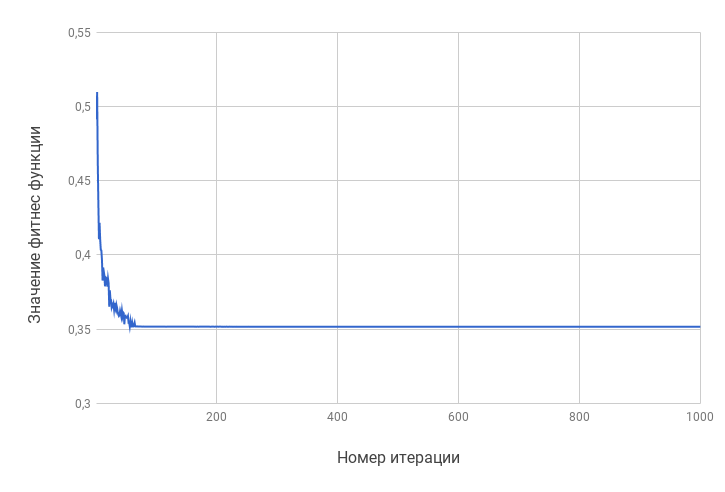
\includegraphics[scale=0.65]{gen_1.png}  
	\caption{Сходимость генетического алгоритма на тестовом наборе}
	\label{fig:gen_1}
\end{figure}

Оптимальное решение при запуске на данном наборе находится на ранних итерациях алгоритма. Следует отметить скорость работы, общее время выполнения не превышало пяти секунд. 

Высокая скорость работы позволяет использовать полученное решение для более широкого класса задач. Одним из вариантов дальнейшего развития системы может являться добавление нового функционала использующего полученный алгоритм в качестве вспомогательного инструмента. Одним из примеров функционала является механизм рекомендаций расположения агентов: система может случайным образом добавлять агента в тестовом окружении и производить расчет эффективности получившегося действия. В случае увеличения показателей может производиться информирование клиента системы о возможности улучшения безопасности системы.

Как можно видеть из гистограммы на рис. \ref{fig:gen_gist_fitness} сходимость подобного рода наблюдается на большинстве сгенерированных тестовых наборов, однако в некоторых случаях оптимальное решение строится на гораздо более поздних итерациях. 

\begin{figure}[!htbp]
\centering
	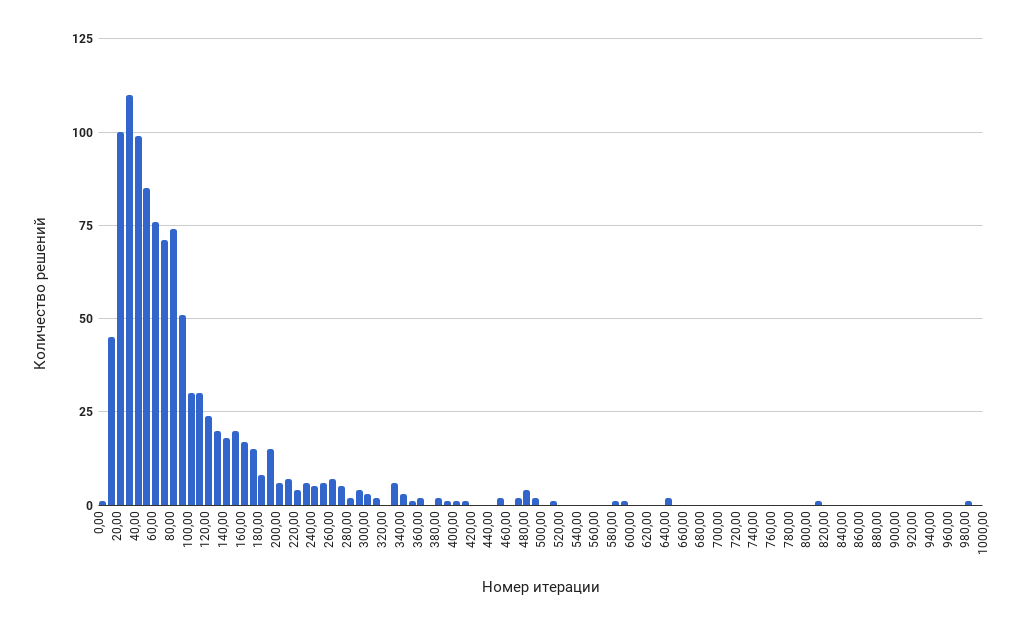
\includegraphics[scale=0.47]{gen_gist_fitness.png}  
	\caption{Гистограмма количества решений по номеру итерации, на котором алгоритм сходился по целевой функции}
	\label{fig:gen_gist_fitness}
\end{figure}

Фактом наличия вариантов с низкой эффективностью алгоритма было решено пренебречь, так как главной задачей остается максимизация вероятности контакта злоумышленника с элементами обманной системы. Решение по данному криетрию достигается на гораздо более ранних итерациях, что демонстрирует гистограмма на рис. \ref{fig:gen_gist_probab}.

\begin{figure}[ht]
\centering
	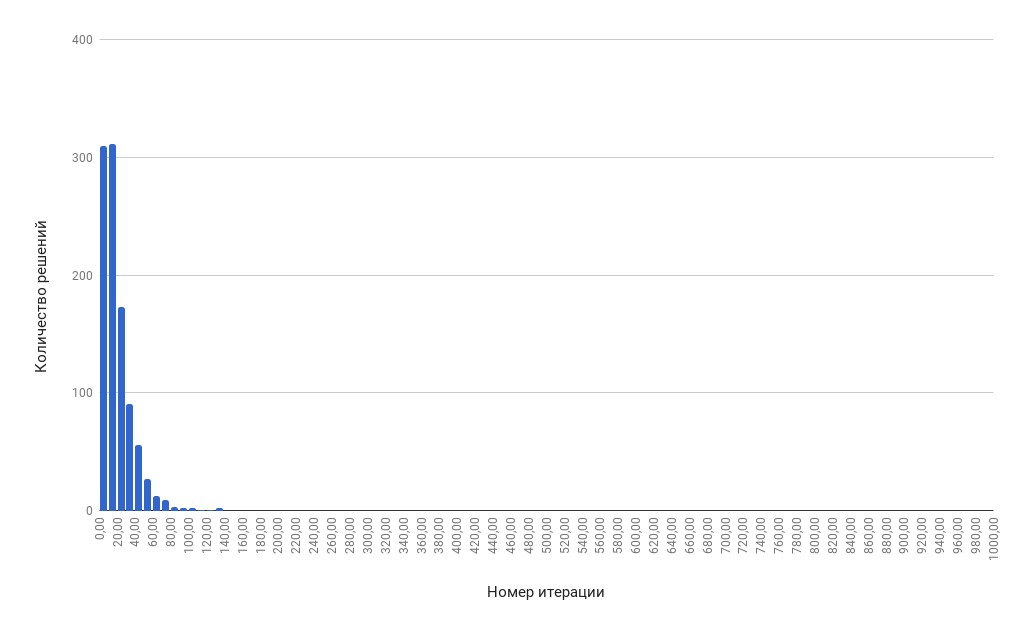
\includegraphics[scale=0.47]{gen_gist_probab.png}  
	\caption{Гистограмма количества решений по номеру итерации, на котором алгоритм сходился по величине $1 - P_{honey, min}$}
	\label{fig:gen_gist_probab}
\end{figure}

\section{Реализация системы автоматического разворачивания ОбС}

По выработанной высокоуровневой архитектуре системы было разработано программное обеспечение, состоящее из двух исполняемых файлов: центральный узел и модуль агента.

\subsection{Реализация центрального узла}

К реализации центрального узла не предъявлялось никаких специфичных технологических требований, вся его деятельность сводится к поддержанию соединения по протоколу \textit{WebSocket} и коммуникации с агентами. По этой причине использовался технологический стек, состоящий из наиболее распространенных, либо наиболее привычных разработчику инструментов:
\begin{itemize}
	\item в качестве языка программирования использовался язык \textit{Kotlin};
	\item для сохранения текущего состояния системы и происходящих событий использовалась \textit{MySQL} база данных;
	\item решение разрабатывалось по принципу инверсии управления с использованием фреймворка \textit{Spring Boot};
	\item для реализации генетического алгоритма использовалась библиотека \textit{jMetal}.
\end{itemize}

Выбор базирующегося на \textit{JVM} языка позволил получить на выходе кроссплатформенное решение, не зависящее от исполняемого окружения, что должно упростить жизнь потенциальным клиентам системы автоматического разворачивания обманной системы, а использование фреймворка \textit{Spring Boot} позволило получить самодостаточный исполняемый \textit{jar} файл, тем самым исключив необходимость установки сервера приложений.

Подключение сторонней библиотеки \textit{jMetal} исключило необходимость реализации выбранного генетического алгоритма \textit{NSGAII}, позволив сконцентрировать внимание на реализации операторов алгоритма. Библиотека существенно упрощает сложность реализации математической части разрабатываемой системы. Процедура получения решения по переданной конфигурации сети представлепна ниже.

\begin{lstlisting}[style=kotlinstyle, label=lst:crossover]
	fun solve(networkConfiguration: NetworkConfiguration) {
	    val honeypotProblem = HoneypotProblem(networkConfiguration, initialSolutionGenerator)
	    //инициализация алгоритма
	    val genetic = NSGAIIBuilder<HoneypotSolution>(honeypotProblem,
	                DistributionCrossover(), 
	                Mutation())
	            .setPopulationSize(100)
	            .setMaxEvaluations(100000)
	            .build()
	    //запуск алгоритма
	    genetic.run()
	    //выбор оптимального решения
	    var distributions = genetic.population.map { it.honeysDistribution }.toList()
	    distributions = distributions.sortedWith(Comparator { a, b ->
	        val r = a.first.compareTo(b.first)
	        return@Comparator if (r != 0) r else a.second.compareTo(b.second)
	    })

	    distributions[0].third.apply(networkConfiguration)
	}
\end{lstlisting}

Работа с центральным узлом происходит посредством \textit{web} интерфейса, который позволяет производить следующие действия:
\begin{itemize}
	\item загружать топологию корпоративной сети посредством конфигурационного файла;
	\item производить добавление агентов в систему;
	\item производить запуск процедуры подбора рекомендуемой конфигурации обманной системы;
	\item вручную модифицировать состояние ловушек на агентах;
	\item просматривать список событий с ловушкек.
\end{itemize}

Для разрабатываемой системы из информации об компьютерной сети требуется только разбиение множества узлов на зоны с одинаковым уровнем доступа. Так как общепринятого формата представления компьютерной сети не существует, то возникает необходимость в создании собственного. Учитывая малые требования к входным данным, системному администратору не должно составить труда сформировать представление в требуемом формате.

Конфигурационный файл системы автоматического разворачивания должен содержать в себе:
\begin{itemize}
	\item множество зон защищаемой сети;
	\item указание зоны, имеющей контакт с внешней сетью. Данный пункт необходим для определения потенциальных маршрутов злоумышленника через защищаемую сеть;
	\item список зон потенциальных целей атак, которые содержат в себе информацию, представляющую интерес для злоумышленника;
	\item информацию возможности передачи информации между заданным множеством зон.
\end{itemize}

Формат конфигурационного файла представлен далее на синтетическом примере.

\begin{lstlisting}[style=gostyle, label=lst:crossover]
	{  
	   //Список зон с одинаковым уровнем доступа
	   "zones":[  
	      {  
	         //Идентификатор зоны. Должен быть уникальным
	         "zone_id":"DMZ",
	         //Список узлов в зоне
	         //Так как разрабатываемая система не использует информацию непосредственно о самих узлах, то в данном списке достаточно передать лишь некоторые идентификаторы узлов, которые могут содержать любую неоходимую для системного администратора информацию, к примеру IP адрес или назначение узла
	         "nodes":[  
	            "dmz1",
	            "dmz2",
	            "dmz3"
	         ]
	      },
	      {  
	         "zone_id":"Рабочая сеть",
	         "nodes":[  
	            "10.0.0.2",
	            "10.0.0.3",
	            "10.0.0.4"
	         ]
	      },
	      {  
	         "zone_id":"Бухгалтерия",
	         "nodes":[  
	            "192.168.0.2",
	            "192.168.0.3",
	            "192.168.0.4(1C БД)"
	         ]
	      }
	   ],
	   //Список критических зон сети с защищаемой информацией
	   "vulnerable_zones":[  
	      "Бухгалтерия"
	   ],
	   //Наименование зоны имеющей контакт с внешней сетью
	   "border_zone":"DMZ",
	   //Список смежности, состоящий из пар идентификаторов зон. Наличие элемента в данном списке говорит о факте возможной передачи информации между указанными зонами.
	   "adjacency":[  
	      {  
	         "zone_id1":"DMZ",
	         "zone_id2":"Рабочая сеть"
	      },
	      {  
	         "zone_id1":"Рабочая сеть",
	         "zone_id2":"Бухгалтерия"
	      }
	   ]
	}
\end{lstlisting}


\subsection{Реализация агента}

Наиболее значимые из выдвигаемых к разрабатываемой системе требований возлагаются на сторону агента, так как непосредственное взаимодействие с ловушкой и контроль действий злоумышленника происходят на его стороне.

Большинство операций, производимых на агенте относятся к категории взаимодействий с \textit{docker} контейнерами. Для управления состояниями контейнеров удаленным образом \textit{Docker} предоставляет программный интерфейс, называемый \textit{Engine} \textit{API}. Так как агент является наиболее важным элементом разрабатываемой системы, то необходимо обеспечить наиболее надежную интеграцию с предоставляемым программным интерфейсом.

Существуют реализации клиентских библиотек, обеспечивающих работу с \textit{Engine API}, практически под все популярные языки программирования, однако факт критичности контекста использования рекомендует выбирать реализации, предоставляемые разработчиками \textit{Docker} и обновляемые с каждым последующим выпуском новой версии системы.

\textit{Docker} предоставляет клиентские библиотеки для двух языков программирования: \textit{Go} и \textit{Python}. Учитывая тот факт, что сам \textit{Docker} реализован на \textit{Go}, следует предполагать, что библиотека на данном языке имеет более качественную поддержку со стороны разработчиков. По данной причине модуль агента разрабатывался на языке программирования \textit{Go}.

Любые действия, производимые пользователем в системе, обязательно затрагивают окружение системы в следующих моментах:
\begin{itemize}
	\item список исполняемых процессов. В случае интерактивного удаленного взаимодействия с системой должна быть запущена, как минимум командная оболочка, таким образом попадание злоумышленника в ловушке сразу отразится на множестве процессов системы;
	\item файловая система. Невозможно представить работу с операционной системой без создания или модифицирования файлов. Действия пользователя влекут за собой создание записей в лог файлах, изменения в журналах событий, злоумышленник может пытаться изменить конфигурацию системы, доставлять вредоносные файлы.
\end{itemize}

Таким образом перечисленные пункты прекрасно подходят на роль индикаторов попадания злоумышленника в ловушку и обязательно долны анализироваться у обслуживаемого контейнера.

Реализованный агент позволяет выполнять следующие действия:
\begin{itemize}
\item производить подключение к центральному узлу системы по протоколу \textit{WebSocket} с использованием \textit{SSL} шифрования;
\item по команде от сервера изменять тип контейнера;
\item производить запуск и остановку контейнера по команде от центрального узла;
\item анализировать изменения в файловой системе контейнера и оповещать сервер в случае возникновения таковых;
\item анализировать изменения в списке запущенных процессов и оповещать сервер в случае возникновения таковых.
\end{itemize}

Процедура анализа изменений в файловой системе, не смотря на кажущуюся сложность, представляет собой достаточно простой процесс благодаря тому, что \textit{Engine API} содержит метод получения списка всех измененных, добавленных или удаленных файлов. Таким образом вся процедура отслеживания сводится к периодическому запуску метода программного интерфейса.

\begin{lstlisting}[style=gostyle]
	changes, err := w.cli.ContainerDiff(*w.ctx, w.containerId)
	if err != nil {
	  w.Hub.Events <- events.Event{Type: events.AgentError, Message: err.Error()}
	}
	var changesStr []string //сериализация изменений
	if len(w.containerState.changedFiles) != 0 && !reflect.DeepEqual(w.containerState.changedFiles, changesStr) {
	  w.Hub.Events <- events.Event{Type: events.MotionDetected, Message: "There is changes in filesystem!"}
	  w.Hub.Events <- events.Event{Type: events.MotionDetected, Message: fmt.Sprint(changesStr)}
	}
\end{lstlisting}

Агент содержит три конфигурационных параметра:
\begin{itemize}
	\item адрес центрального узла;
	\item относительный путь для \textit{websocket} подключения;
	\item абсолютный путь расположения корневого сертификата для \textit{SSL} шифрования;
	\item секрет для аутентификации при установке соединения с центральным узлом.
\end{itemize}

Конфигурационные параметры передаются через аргументы командной строки.

Агент не хранит своего состояния и получает его при установке соединения с центральным узлом.

% Зачем: Изменение надписи для списка литературы
% Почему: Пункт 2.8.1 Требований по оформлению пояснительной записки.
\renewcommand{\bibsection}{\sectioncentered*{Cписок использованных источников}}
\phantomsection\pagebreak% исправляет нумерацию в документе и исправляет гиперссылки в pdf
\addcontentsline{toc}{section}{Cписок использованных источников}

% Зачем: Печать списка литературы. База данных литературы - файл bibliography_database.bib
\bibliography{bibliography_database}


% \includepdf позволяет включить в результирующий pdf документ часть другого pdf документа, сделанного
% например не с помощью TeX. Бывает полезно, если какие-то диаграммны нарисованы, например, с помощью 
% Microoft Office и сохранены в pdf.
%\includepdf[pages={-}]{documents_list.pdf}

\end{document}